% secuencia de comunicacion SPS30 
	\shorthandoff{>}
	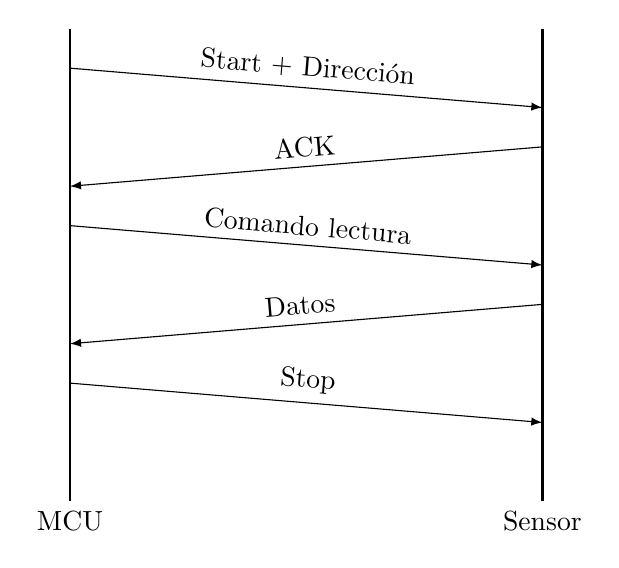
\begin{tikzpicture}[
	node distance=2cm,
	every node/.style={align=center},
	label/.style={draw=none}
	]
	% Líneas de tiempo verticales
	\draw[thick] (0,0) -- (0,-6) node[below] {MCU};
	\draw[thick] (6,0) -- (6,-6) node[below] {Sensor};
	
	% Mensajes
	\draw[-latex] (0,-0.5) -- (6,-1) node[midway, above, sloped] {Start + Dirección};
	\draw[-latex] (6,-1.5) -- (0,-2) node[midway, above, sloped] {ACK};
	\draw[-latex] (0,-2.5) -- (6,-3) node[midway, above, sloped] {Comando lectura};
	\draw[-latex] (6,-3.5) -- (0,-4) node[midway, above, sloped] {Datos \MPF};
	\draw[-latex] (0,-4.5) -- (6,-5) node[midway, above, sloped] {Stop};
	\end{tikzpicture}
	\shorthandon{>}